\begin{frame}{Theme}

\begin{figure}
	\centering
	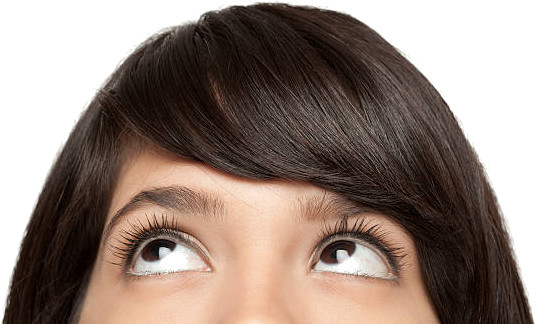
\includegraphics[scale=0.20]{res/images/temi}
\end{figure}

\begin{itemize}
	\item Si parla di temi invece nel caso di presentazioni \texttt{beamer}
	\item Anche in questo caso è possibile definirne uno proprio ma non lo
	faremo
	\item È possibile applicare un tema usando il comando
	\texttt{\textbackslash{}usetheme\{nome\_pacchetto\}}
	\item Certi temi permettono di scegliere la gamma di colori sfruttando il
	comando \texttt{\textbackslash{}usecolortheme\{nome\_colore\}}
\end{itemize}

\end{frame}